\documentclass[10pt]{article}

\usepackage[a4paper,margin=2cm]{geometry}
\usepackage{amsmath}
\usepackage{graphicx}
\usepackage{subcaption}
\usepackage{float}
\usepackage[hidelinks]{hyperref}

% the figures live in the figures/ folder next to this file
\graphicspath{{figures/}{../figures/}{./}}

\setlength{\parskip}{2pt}
\setlength{\parindent}{0pt}

\title{\vspace{-1.2cm}Computer Programming Assignment 2025\\ \large MCMC sampling of the 2D Ising model}
\author{Matteo Medini}
\date{}

\begin{document}
\maketitle
\vspace{-0.8cm}

\section{Setup}
We study the 2D Ising model on an $N\times N$ square lattice with periodic boundary
conditions. Each spin $s_i \in \{-1,+1\}$ and the energy is
\[
H(s) = -\tfrac{1}{2}\sum_i \sum_{j\in N(i)} J_{ij}\, s_i s_j , \qquad J_{ij}=1 .
\]
Configurations are sampled from the Boltzmann distribution $P(s)\propto e^{-\beta H(s)}$
with a Metropolis single spin flip chain: we pick a site at random, propose $s_i\to-s_i$,
and accept with probability $\min\{1,e^{-\beta\Delta H}\}$, where
$\Delta H = 2 s_i \sum_{j\in N(i)} s_j$. The relevant observables are the magnetization
per spin $m(s)=\frac{1}{N^2}\sum_i s_i$, the energy, and the cluster sizes.

\section{Task 1: completing the code}
\textbf{cost().} With periodic boundaries every spin owns one right and one down bond, so
summing only those two directions already covers all bonds exactly once. Using
\texttt{np.roll} for the shift, the energy is just minus the sum of the right and down
nearest neighbour products. This is fully vectorised and avoids any Python loop.

\textbf{compute\_delta\_cost().} A single flip only changes the four bonds attached to the
chosen site, so $\Delta H = 2 s_i (s_{up}+s_{down}+s_{left}+s_{right})$, with the modulo
taking care of the boundaries. This is $O(1)$ and matches a full recomputation of the cost
(checked with the \texttt{debug\_delta\_cost} flag of \texttt{mcmc.py}).

\textbf{find\_clusters().} We follow Algorithm 1: a flood fill that grows a cluster from a
seed, visiting the four neighbours and keeping the ones with the same spin. We replaced the
per cluster \texttt{np.random.choice} seed search (which scans the whole mask every time)
with a single advancing index. The list of cluster sizes does not depend on the seed order,
so this keeps the routine close to $O(N^2)$ even when there are thousands of small clusters.

\section{Task 2: exploring the MCMC parameters}

\begin{figure}[H]
\centering
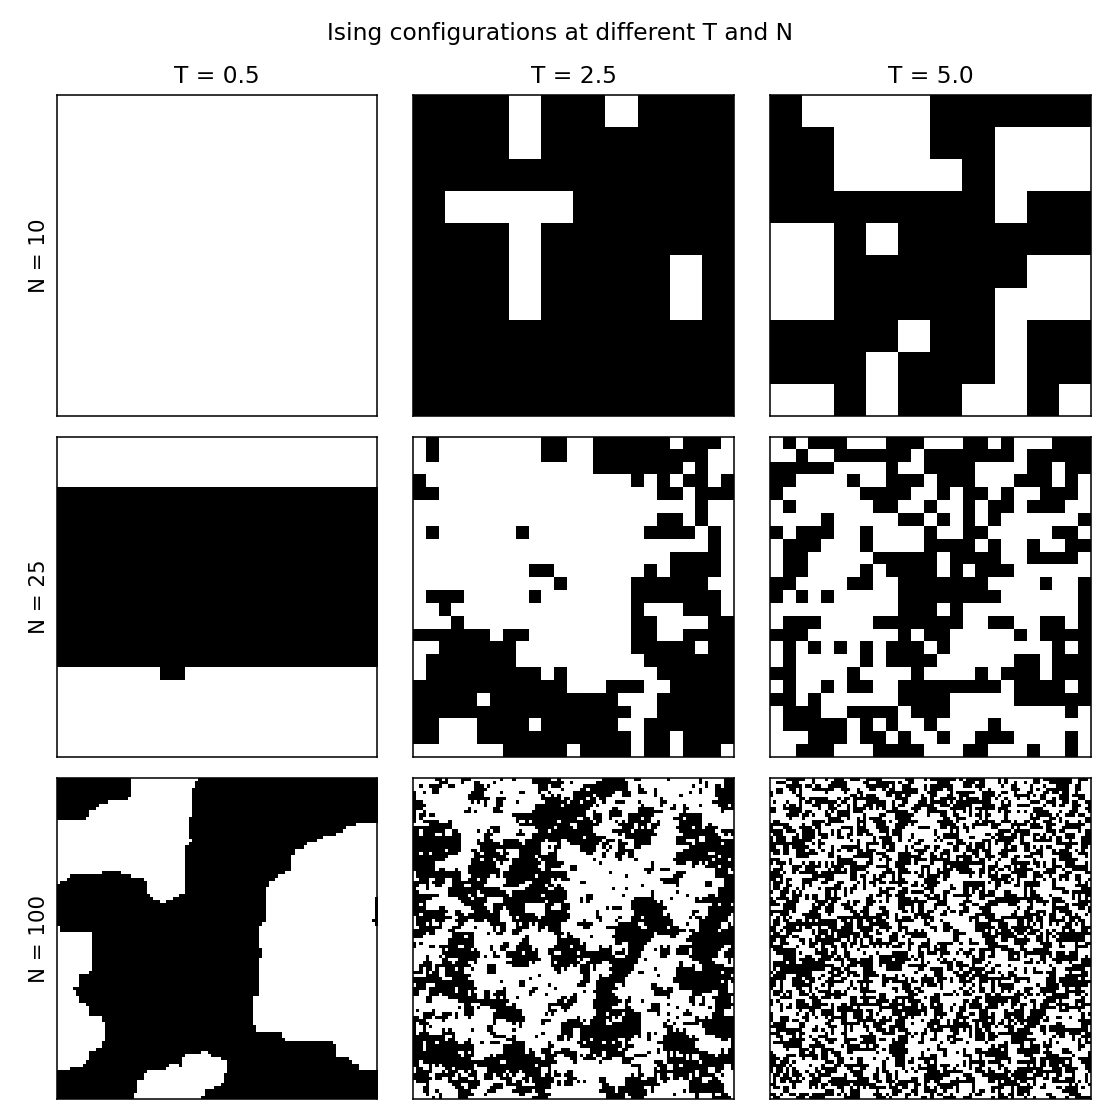
\includegraphics[width=0.62\textwidth]{snapshots.png}
\caption{Configurations after burn in (positive spins in black). Columns are
$T\in\{0.5,2.5,5.0\}$, rows are $N\in\{10,25,100\}$.}
\label{fig:snap}
\end{figure}

Figure \ref{fig:snap} shows that aligned spins are only seen at low temperature. At $T=0.5$
the lattice is essentially uniform (the $N=25$ panel is caught in a long lived two domain
stripe, see the burn in discussion below). At $T=5.0$ the configuration is a random salt and
pepper pattern with no order. Clusters, meaning extended domains of equal spin that are
neither tiny nor system spanning, appear around $T=2.5$, which is close to the critical
temperature $T_C\simeq 2.27$. There the $N=100$ panel shows the characteristic mix of
domains of every size.

\begin{figure}[H]
\centering
\begin{subfigure}{0.49\textwidth}
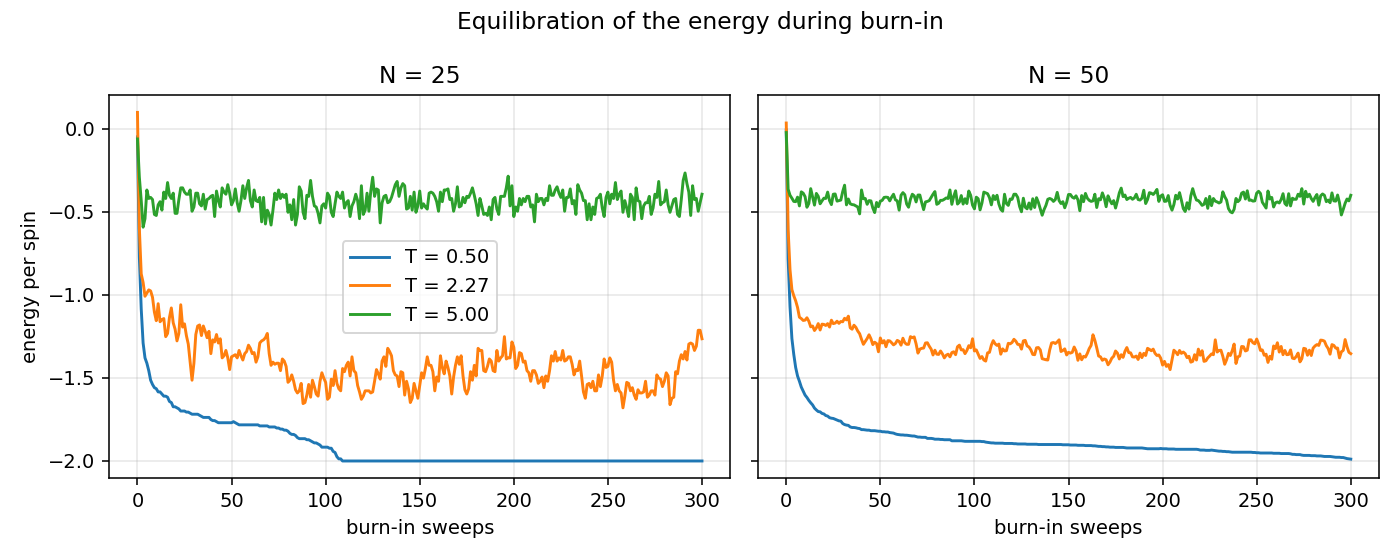
\includegraphics[width=\textwidth]{burnin.png}
\end{subfigure}
\hfill
\begin{subfigure}{0.49\textwidth}
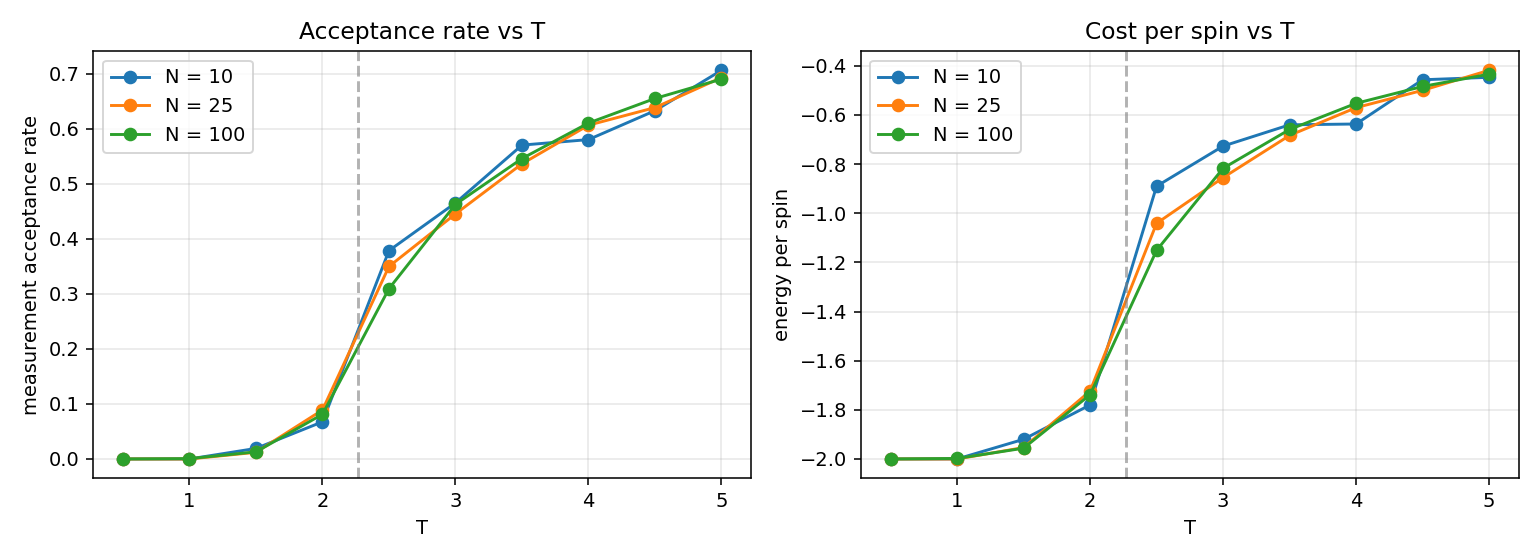
\includegraphics[width=\textwidth]{acceptance_cost.png}
\end{subfigure}
\caption{Left: energy per spin during burn in for three temperatures and two sizes.
Right: measurement acceptance rate and energy per spin versus $T$ for the three $N$.
The dashed line marks $T_C$.}
\label{fig:burn}
\end{figure}

The acceptance rate (Fig. \ref{fig:burn}, right) grows with $T$: at low $T$ almost every
flip raises the energy and is rejected, while at high $T$ roughly $70\%$ of the flips are
accepted. The energy per spin rises from the ground state value $-2$ at low $T$ towards $0$
at high $T$. Away from $T_C$ both quantities depend very weakly on $N$, the only visible
difference is that the small $N=10$ system is noisier.

The minimal burn in needed for a roughly constant cost clearly depends on both $T$ and $N$.
At high $T$ the energy reaches its plateau in a handful of sweeps. At low $T$ it takes longer
because the system has to grow a single domain, and for the larger lattice it relaxes more
slowly. The hardest case is near $T_C$: the energy keeps fluctuating with large amplitude
and never settles to a sharp value, which is the well known critical slowing down. In
practice we used a burn in of the order of one hundred to a few hundred lattice sweeps (one
sweep equals $N^2$ proposed flips), with the longer values reserved for temperatures near
$T_C$ and for the larger lattices.

\section{Task 3: statistical properties and critical temperature}
For this part we fixed $N=32$, used a cold (ordered) start to avoid the striped metastable
states that trap the chain below $T_C$, and pooled $3$ independent chains with a longer wait
near $T_C$ (where samples are strongly correlated). We scanned $\beta$ from $0.1$ to $1.0$
with a finer spacing around $\beta_c$.

\begin{figure}[H]
\centering
\begin{subfigure}{0.49\textwidth}
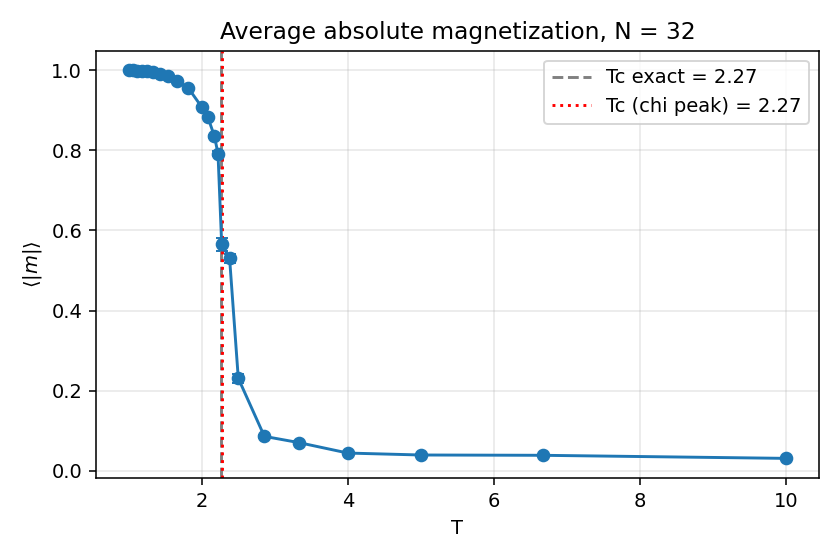
\includegraphics[width=\textwidth]{magnetization.png}
\end{subfigure}
\hfill
\begin{subfigure}{0.49\textwidth}
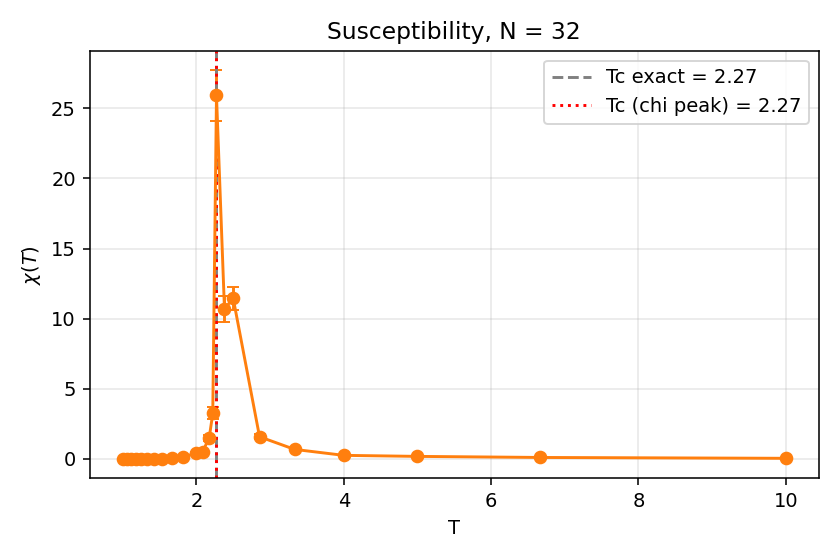
\includegraphics[width=\textwidth]{susceptibility.png}
\end{subfigure}
\caption{Average absolute magnetization and finite size susceptibility versus $T$ for
$N=32$. The exact $T_C=2.269$ and the susceptibility peak are marked.}
\label{fig:magchi}
\end{figure}

\textbf{Critical temperature.} The magnetization $\langle|m|\rangle$ (Fig. \ref{fig:magchi},
left) stays close to $1$ in the ordered phase and drops quickly around $T\simeq 2.3$. Reading
$T_C$ as the highest $T$ where $\langle|m|\rangle$ is still clearly above its finite size
floor gives about $2.5$. The susceptibility (right) is much sharper: it has a clear peak at
$T_C\simeq 2.27$, in excellent agreement with the exact value $2.269$. We adopt the
susceptibility estimate as our value of $T_C$, since on a finite lattice the peak position is
a cleaner estimator than the magnetization onset.

\begin{figure}[H]
\centering
\begin{subfigure}{0.49\textwidth}
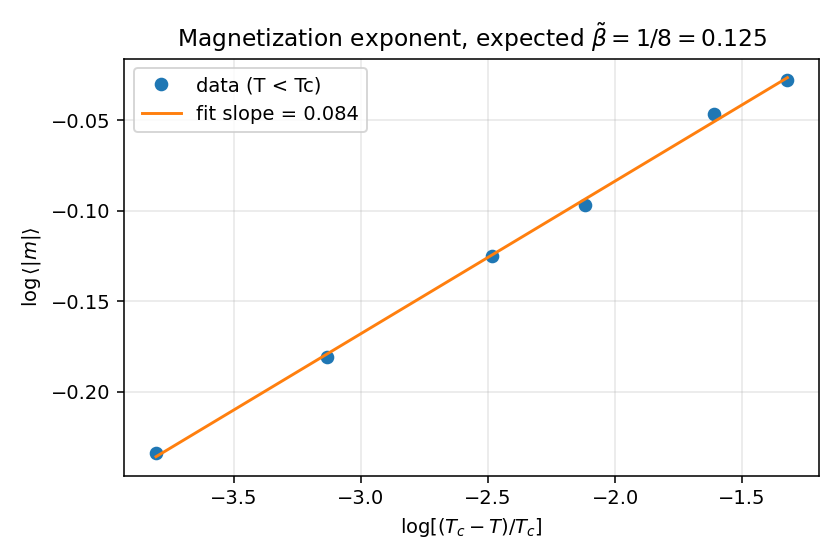
\includegraphics[width=\textwidth]{fit_beta.png}
\end{subfigure}
\hfill
\begin{subfigure}{0.49\textwidth}
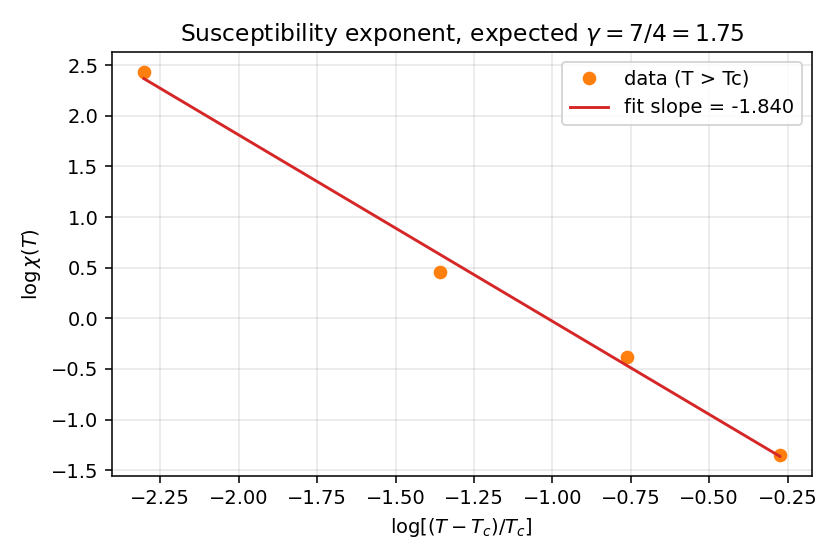
\includegraphics[width=\textwidth]{fit_gamma.png}
\end{subfigure}
\caption{Power law fits. Left: $\log\langle|m|\rangle$ versus $\log[(T_C-T)/T_C]$ for
$T<T_C$. Right: $\log\chi$ versus $\log[(T-T_C)/T_C]$ for $T>T_C$.}
\label{fig:fits}
\end{figure}

\textbf{Critical exponents.} Fitting the magnetization below $T_C$ (Fig. \ref{fig:fits},
left) gives a slope $\tilde\beta\simeq 0.084$, to be compared with the exact $1/8=0.125$.
The susceptibility above $T_C$ (right) gives $\gamma\simeq 1.84$, close to the exact
$7/4=1.75$. The susceptibility exponent comes out well, while $\tilde\beta$ is underestimated.
This is expected: on a small lattice the magnetization is rounded near $T_C$, and the fit is
very sensitive to the value of $T_C$ used (a slightly higher effective critical temperature
would push the slope towards $1/8$). We kept the same $T_C$ for both fits to stay consistent.
A larger lattice and longer runs would tighten both estimates.

\textbf{Cluster sizes.} Figure \ref{fig:clusters} shows the cluster size distribution at the
three temperatures for $N\in\{10,50,100,200\}$, on log log axes. At $T=0.5$ there is a single
cluster covering the whole lattice (one point at size $N^2$). At $T=5.0$ there are many small
clusters and the distribution falls off fast, with a cutoff at small sizes. Around $T_C$ the
picture changes completely: the distribution becomes broad and roughly straight on log log
axes, that is approximately scale free, and a single spanning cluster appears (for $N=200$ it
already reaches about half of the lattice). This is the cluster signature of the transition:
domains of all sizes coexist and the system is on the verge of percolating, which is exactly
what makes $T_C$ special.

\begin{figure}[H]
\centering
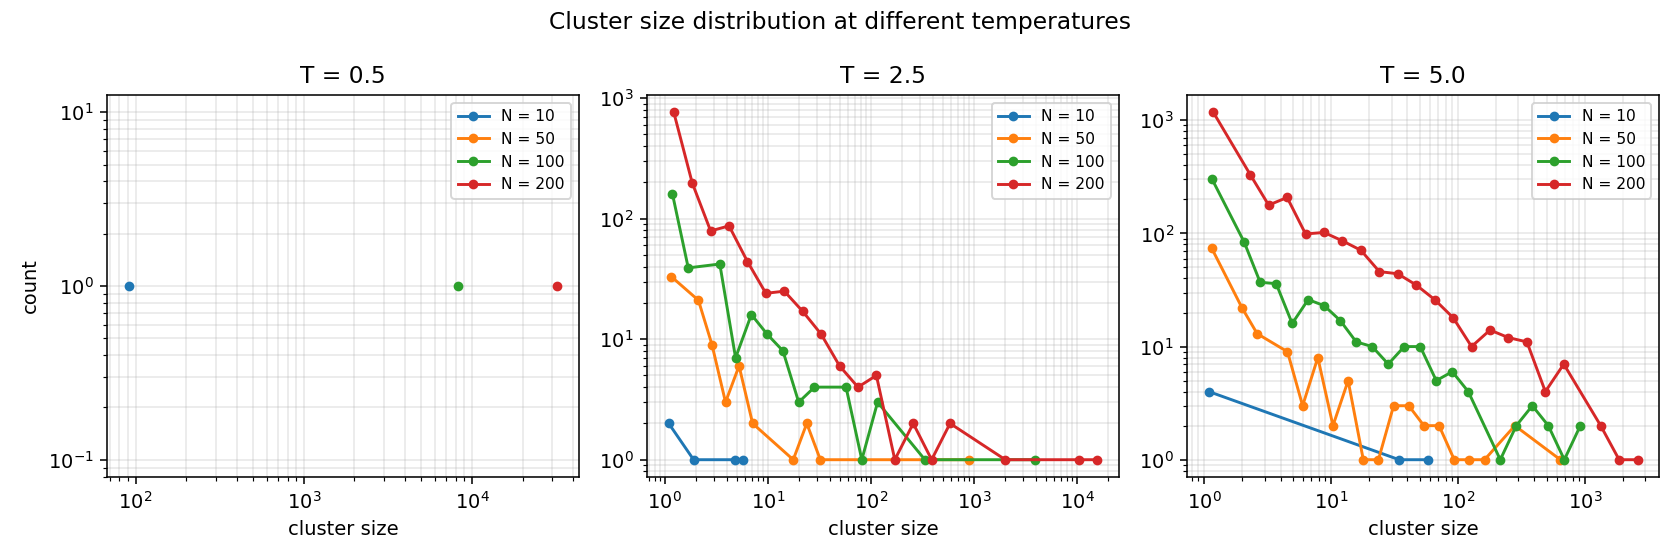
\includegraphics[width=0.95\textwidth]{clusters.png}
\caption{Cluster size distribution at $T\in\{0.5,2.5,5.0\}$ for several $N$ (log log axes).}
\label{fig:clusters}
\end{figure}

\section{Conclusions}
The single spin flip Metropolis sampler reproduces the two phases of the 2D Ising model and
locates the critical temperature accurately from the susceptibility peak ($T_C\simeq 2.27$
against the exact $2.269$). The critical exponents come out as $\gamma\simeq 1.84$ (exact
$1.75$) and $\tilde\beta\simeq 0.08$ (exact $0.125$), the magnetization exponent being the
harder one to measure on a finite lattice. The choice of parameters matters a lot: a cold
start removes metastable stripes below $T_C$, and a long wait near $T_C$ is needed because of
critical slowing down. The cluster analysis gives a clean and intuitive view of the
transition, from one giant domain at low $T$, to a broad scale free distribution at $T_C$, to
many small islands at high $T$.

\end{document}
